\documentclass[conference]{IEEEtran}
\IEEEoverridecommandlockouts

\usepackage{cite}
\usepackage{graphicx}
\usepackage{amsmath}
\usepackage{booktabs}
\usepackage{multirow}
\usepackage{url}
\usepackage{xcolor}
\usepackage{balance}

\title{ResearchLanka AI: A Provenance-Aware, Human-in-the-Loop Pipeline for Mapping Sri Lankan Artificial Intelligence Research}

\author{\IEEEauthorblockN{Anusank Krishnathas}
\IEEEauthorblockA{ResearchLanka AI Project, Sri Lanka\\
\url{https://github.com/krish-anu/researchlanka-ai}}}

\begin{document}
\maketitle

\begin{abstract}
National research maps are difficult to construct when institutional repositories, global indexes, and publisher registries disagree on identity, affiliation, document version, and subject relevance. We present ResearchLanka AI, a reproducible data pipeline and analytics platform for identifying artificial-intelligence (AI) scholarship with supported Sri Lankan ownership. The system integrates OpenAlex, Crossref, Sri Lanka Journals Online, and institutional repositories; maps heterogeneous records to a common schema; applies conservative ownership rules; consolidates versions; and routes uncertain AI classifications to human review. The resulting release contains 3,555 distinct works from 2016--2026, 11,585 parsed author-name strings, and 50 normalized Sri Lankan institutions. DOI, keyword, and abstract availability are 99.1\%, 95.0\%, and 81.5\%, respectively. Sixty percent of works have corroborating metadata from more than one source. A release audit resolved 214 uncertain AI decisions, rejected 47 records supported only by ambiguous institution aliases, and consolidated 95 version groups by removing 107 alternate records. The platform exposes the curated corpus through a versioned dataset, read-only API, and interactive dashboard while preserving row-level provenance. We describe the engineering decisions, validation evidence, corpus characteristics, and remaining threats to validity. The principal contribution is not a benchmark classifier, but an auditable national-scale workflow that separates high-confidence automation from decisions requiring human judgement.
\end{abstract}

\begin{IEEEkeywords}
bibliometrics, scholarly metadata, artificial intelligence, Sri Lanka, data integration, human-in-the-loop, research analytics
\end{IEEEkeywords}

\section{Introduction}
Quantitative maps of research activity support funding, collaboration, institutional strategy, and science policy. Their usefulness, however, depends on the less visible work of identifying the same publication across sources, resolving affiliation evidence, and distinguishing genuine field contributions from records that merely contain fashionable terminology. Science-of-science research has made large-scale scholarly analysis increasingly feasible~\cite{fortunato2018science}, while modern open infrastructures provide broad programmatic access to research metadata. Yet source coverage and completeness vary by document type and discipline~\cite{visser2021comparison}. These limitations are especially consequential for national and regional maps, where a single ambiguous institution alias or missed local repository can materially change an institution's apparent output.

ResearchLanka AI addresses this problem for AI-related scholarship connected to Sri Lanka. It is both a data-processing system and a public-facing analytics application. Rather than treating a country filter or keyword query as ground truth, the system records source evidence, imposes a separate Sri Lanka ownership gate, classifies AI relevance with an uncertainty band, and retains a decision trail for human adjudication. The work makes three contributions:
\begin{itemize}
  \item an extensible collection and normalization pipeline spanning global indexes, publisher metadata, and local repositories;
  \item an auditable curation procedure combining deterministic validation, version-aware deduplication, conservative ownership rules, and human review; and
  \item a characterized 3,555-work corpus and deployable analytics stack comprising a versioned CSV, PostgreSQL schema, read-only API, and web dashboard.
\end{itemize}

This paper reports the state of the canonical version 1.0 CSV on 20 October 2026. The 2026 count is therefore partial. We intentionally do not present the operational review labels as an independently blinded machine-learning benchmark.

\section{Related Work}
Bibliometric studies commonly depend on Scopus or Web of Science, but licensing and coverage constraints complicate reproducible, locally maintainable systems. Comparisons of major bibliographic sources demonstrate meaningful differences in coverage, document typing, and citation links~\cite{visser2021comparison}; curated indexes themselves also require continuing duplicate and metadata quality programs~\cite{baas2020scopus}. Methodological guidance consequently emphasizes transparent data retrieval, cleaning, and analysis decisions~\cite{donthu2021bibliometric}.

OpenAlex provides an openly accessible knowledge graph of works, authors, venues, institutions, and concepts~\cite{priem2022openalex}. Crossref exposes publisher-deposited metadata, including identifiers, licences, abstracts, and update relationships, through a public REST API~\cite{crossrefapi}. Local repositories frequently expose Dublin Core or richer records through OAI-PMH, an application-independent harvesting protocol~\cite{oaipmh}. ResearchLanka AI uses these sources as complementary evidence rather than assuming any one source is complete.

Persistent identifiers improve entity resolution: DOI anchors publication matching, while ORCID can distinguish researchers~\cite{haak2012orcid}. Identifiers are nevertheless incomplete, and separate records may represent a preprint, repository copy, conference paper, or journal extension of one work. Our workflow therefore combines identifier matching with normalized-title and year checks, followed by explicit canonical-version selection. The data package follows the spirit of FAIR stewardship~\cite{wilkinson2016fair} through machine-readable schemas, provenance, checksums, and citation metadata, although public redistribution remains subject to final source-rights and dataset-licence approval.

\section{System Design and Method}
\subsection{Architecture and Collection}
Figure~\ref{fig:pipeline} summarizes the pipeline. Collectors ingest OpenAlex, Crossref, Sri Lanka Journals Online (SLJOL), and institutional repositories through REST, OAI-PMH, DSpace, sitemap, and HTML-metadata adapters. Source-specific records are stored before transformation so that parsing logic can be rerun without recollection. A registry describes repository endpoints and institution mappings, permitting new institutions to be added through configuration.

\begin{figure*}[t]
  \centering
  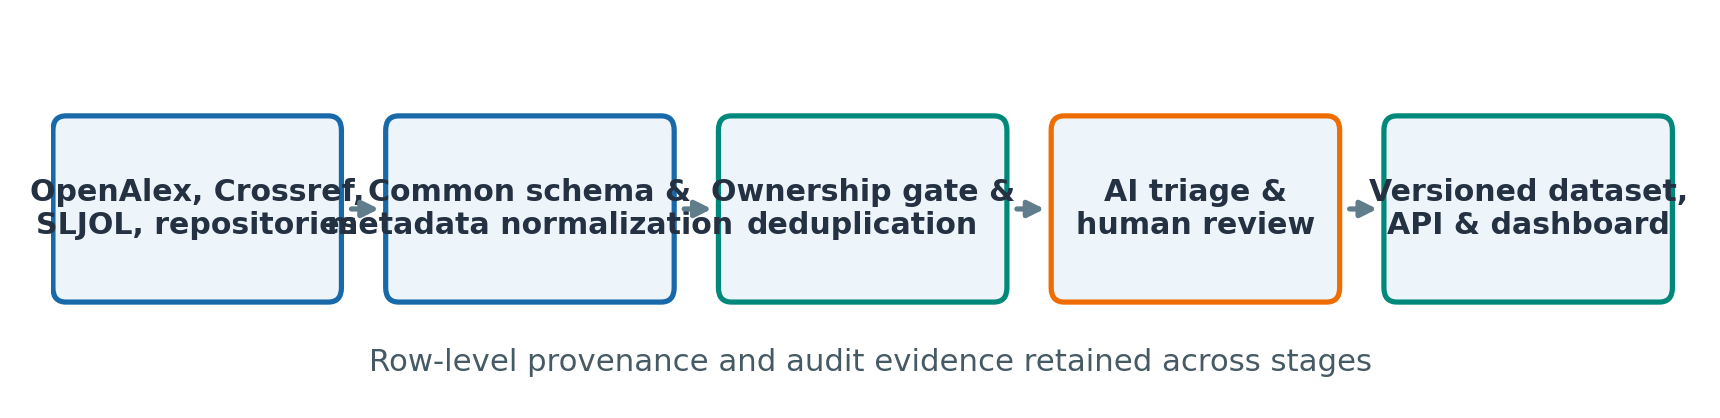
\includegraphics[width=0.97\textwidth]{figures/pipeline.png}
  \caption{ResearchLanka AI pipeline. Automated decisions retain provenance; ambiguous ownership, duplicate-version, and AI-relevance cases enter review rather than being silently accepted.}
  \label{fig:pipeline}
\end{figure*}

All inputs are mapped to a common publication schema. Normalization covers DOI and OpenAlex identifiers, dates, titles, author lists, affiliations, institutions, venues, open-access status, research topics, and document types. Multivalued public fields are serialized with semicolons. The public schema exposes 35 research-facing columns; the private processing master retains 86 columns, including model scores, review provenance, ownership diagnostics, search-normalized text, and missingness flags.

\subsection{Sri Lanka Ownership Gate}
A work must independently pass Sri Lanka ownership rules before publication. Evidence includes normalized Sri Lankan affiliations and author--institution relationships. International collaboration is allowed, but venue location, appearance in a Sri Lankan repository, or a weak first-author name match is not sufficient by itself. Ambiguous aliases are marked for review. The final dataset distinguishes domestic works from Sri Lanka-owned international collaborations and stores the decision class and supporting evidence in the internal master.

This conservative rule prevents a frequent bibliometric failure mode: discovery-source membership being mistaken for intellectual or institutional ownership. A focused validation against an official 24-person academic roster at one department illustrates the policy. That audit verified 299 distinct publications, held four uncertain attributions, and rejected one reviewed misattribution; initials-only matches were never automatically verified. This departmental exercise validates precision-oriented matching behavior but is not a national recall estimate.

\subsection{Deduplication and Version Resolution}
The pipeline first normalizes DOI strings and titles, then constructs candidate groups using OpenAlex ID, DOI, normalized title, and title--year keys. Within a connected group, canonical selection favors a complete, well-identified scholarly record while merging compatible source provenance. Potential preprint/published, repository/publisher, supplement, malformed-DOI, and alternate-version relations are reviewed when deterministic rules cannot safely choose.

The release-readiness audit examined 95 connected title/version groups containing 202 records. It retained 95 canonical works and removed 107 alternatives. The resulting dataset has no repeated nonempty DOI, OpenAlex ID, normalized title, or normalized title--year key. This is a distinct-work policy: it supports corpus-level counting, but it intentionally does not model the full evolution of each manuscript.

\subsection{AI Relevance and Human Review}
AI relevance is implemented as a three-way routing decision:
\begin{equation}
d(p)=\begin{cases}
\textsc{Auto-AI}, & p\geq 0.66,\\
\textsc{Review}, & 0.40<p<0.66,\\
\textsc{Auto-Non-AI}, & p\leq 0.40,
\end{cases}
\end{equation}
where $p$ is produced by an XGBoost text classifier~\cite{chen2016xgboost} using title, abstract, and keywords. Rules derived from observed hard negatives can demote an apparent positive to review when language such as ``smart,'' generic forecasting, signal processing, or statistical modelling appears without explicit AI evidence.

The current model manifest fixes its identifier, feature contract, thresholds, training-data name, artifact path, and SHA-256 checksum. However, the released corpus combines decisions from earlier linear SVM processing, the present model family, LLM-assisted review, and finished human adjudication. Historical reviewers were not consistently blinded to predictions, and agreement metadata are incomplete. We therefore report the classifier only as workflow infrastructure, not as a generalization result. All 214 records remaining in the secondary review queue were adjudicated: 203 were retained as AI, five failed ownership, five were duplicate versions, and one failed both AI and ownership requirements.

\subsection{Serving and Reproducibility}
Accepted records load into PostgreSQL and are exposed through a read-only versioned API. A Next.js interface supports publication search, institution and researcher exploration, topics, collaboration networks, exports, and visible data-quality summaries. Administrative routes support incremental updates and review. Pipeline stages can run locally, in Docker, or as scheduled cloud jobs. The release package includes a data dictionary, methodology, quality report, audit tables, checksums, and citation metadata. Automated project verification reports 786 passing backend tests (12 skipped), 228 passing frontend tests, static checks, and a production web build.

\subsection{Validation Contract}
Validation is treated as an executable release contract rather than a final visual inspection. The validator checks schema identity, identifier uniqueness, required-field population, decision closure, model provenance, and consistency between human-readable and normalized search fields. In particular, a releasable row must have a nonblank title, parseable publication date, source dataset and source record identifier, supported ownership decision, final AI label, model or review provenance, and a confidence value or explicit human-review marker. Dataset-level checks require the exact 35-column public schema, unique OpenAlex identifiers, unique nonempty DOIs, no normalized-title collision, and no unresolved review flag.

The checks are deliberately layered. A syntactically valid DOI does not prove that it belongs to the title; a unique title does not prove valid ownership; and an AI prediction does not prove either bibliographic identity or national relevance. Consequently, automated checks are followed by review artifacts that preserve the candidate record, final disposition, and a short reason. Release files also carry a SHA-256 manifest so that downstream analysis can verify that it used the reviewed bytes. A failure in any mandatory gate stops publication rather than silently dropping the failing assertion.

Several aggregate values are recomputed directly from the canonical CSV during paper preparation. Publication year is derived from the heterogeneous but ISO-like date string; multivalued author and institution fields are split on the documented semicolon delimiter; and percentages use all 3,555 rows unless stated otherwise. The accompanying figure script performs the year and field aggregations from the same file. This design limits transcription drift between the dataset, quality report, figures, and manuscript.

\subsection{Incremental Update Semantics}
The production workflow supports full reconstruction and incremental refresh. Incremental collection stores a checkpoint for each source, maps new candidates through the same common schema, then applies cleaning, ownership, deduplication, and AI-routing policies before loading. A record absent from a later source response is not immediately deleted: retirement is explicit because repository downtime and pagination failure can resemble deletion. Author-contributed corrections are stored separately and merged into a public-eligible database view, preventing a pipeline reload from overwriting reviewed changes. Author-submitted publications likewise require administrative confirmation of both AI relevance and Sri Lanka ownership.

Idempotence is important for scheduled operation. Stable source identifiers and normalized matching keys let a repeated harvest update an existing work instead of inflating counts. Database migrations version structural changes; batch loading occurs after validation; and the read-only public API isolates analytical consumers from administrative state. The system records the model identifier and decision source with each accepted record, allowing a later model change to identify which rows require rescoring. These controls do not make external metadata immutable, but they make changes attributable.

\section{Corpus Results}
\subsection{Scale, Growth, and Coverage}
Table~\ref{tab:quality} describes the canonical corpus. It contains 3,555 distinct publications between 2016 and the partial 2026 snapshot. Parsed semicolon-separated fields yield 11,585 unique author-name strings and 50 normalized Sri Lankan institution labels. These are metadata entities, not fully disambiguated people: a person may occur under multiple printed names.

\begin{table}[t]
\caption{Canonical v1.0 corpus and validation summary.}
\label{tab:quality}
\centering
\small
\begin{tabular}{lr}
\toprule
Measure & Value \\
\midrule
Distinct publications & 3,555 \\
Publication years & 2016--2026 \\
Public / internal columns & 35 / 86 \\
Unique author-name strings & 11,585 \\
Normalized Sri Lankan institutions & 50 \\
DOI available & 3,523 (99.1\%) \\
Abstract available & 2,896 (81.5\%) \\
Keywords available & 3,378 (95.0\%) \\
Multiple-source provenance & 2,134 (60.0\%) \\
Open-access status other than closed & 936 (26.3\%) \\
Domestic / owned international & 3,363 / 192 \\
Unresolved secondary review cases & 0 \\
Residual identifier/title duplicates & 0 \\
\bottomrule
\end{tabular}
\end{table}

Annual output grows from 68 works in 2016 to 660 in 2025 (Fig.~\ref{fig:annual}), a descriptive compound annual growth rate of 28.7\%. This should not be interpreted solely as growth in research activity: later-year discovery, source expansion, repository onboarding, and changing indexing practices also affect the curve. The 582 records assigned to 2026 are partial and may also include online-first metadata.

\begin{figure}[t]
  \centering
  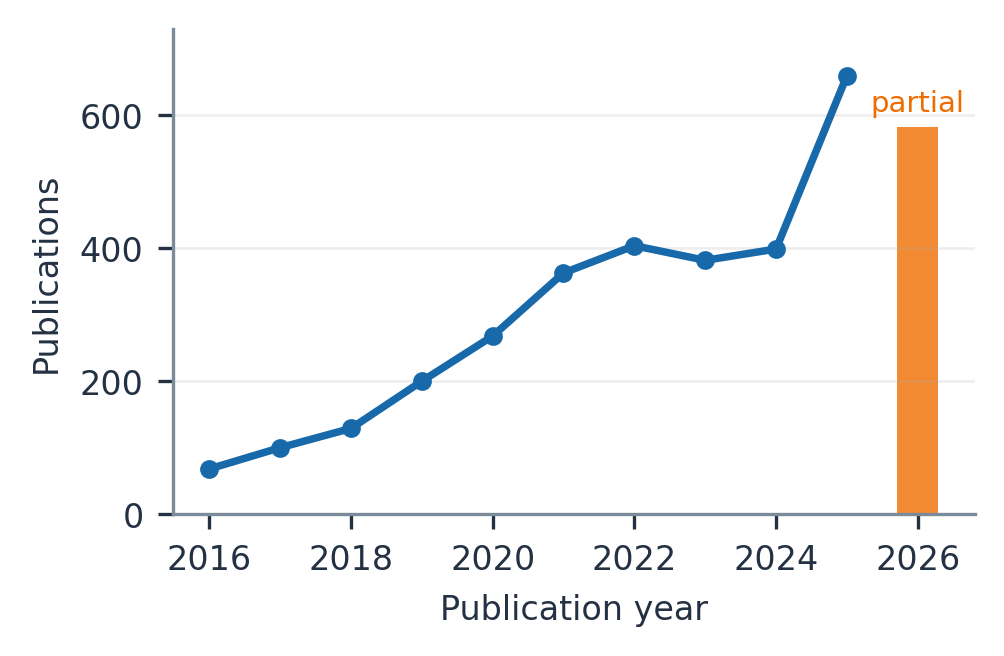
\includegraphics[width=\columnwidth]{figures/annual_output.png}
  \caption{Annual works in the curated corpus. The 2026 bar is a partial-year snapshot and is not used to infer decline.}
  \label{fig:annual}
\end{figure}

Cross-source corroboration is substantial: 1,421 works have OpenAlex-only provenance, while 2,134 (60.0\%) include at least one additional source. The largest merged group is OpenAlex plus Crossref (1,327); repository evidence contributes to 634 merged records, and SLJOL to 149. Provenance counts indicate metadata contribution, not independent confirmation of every individual field.

\subsection{Research and Publication Composition}
Computer Science accounts for 1,588 works (44.7\% of the full corpus), followed by Engineering (437; 12.3\%), Medicine (292; 8.2\%), Psychology (173; 4.9\%), and Agricultural and Biological Sciences (173; 4.9\%). Seventy-four works lack a primary-field value. Figure~\ref{fig:fields} shows the broader disciplinary distribution. The leading subfields are Artificial Intelligence (720), Computer Vision and Pattern Recognition (345), Information Systems (175), and Plant Science (151), illustrating that an AI corpus crosses the boundaries of the Computer Science field label.

\begin{figure}[t]
  \centering
  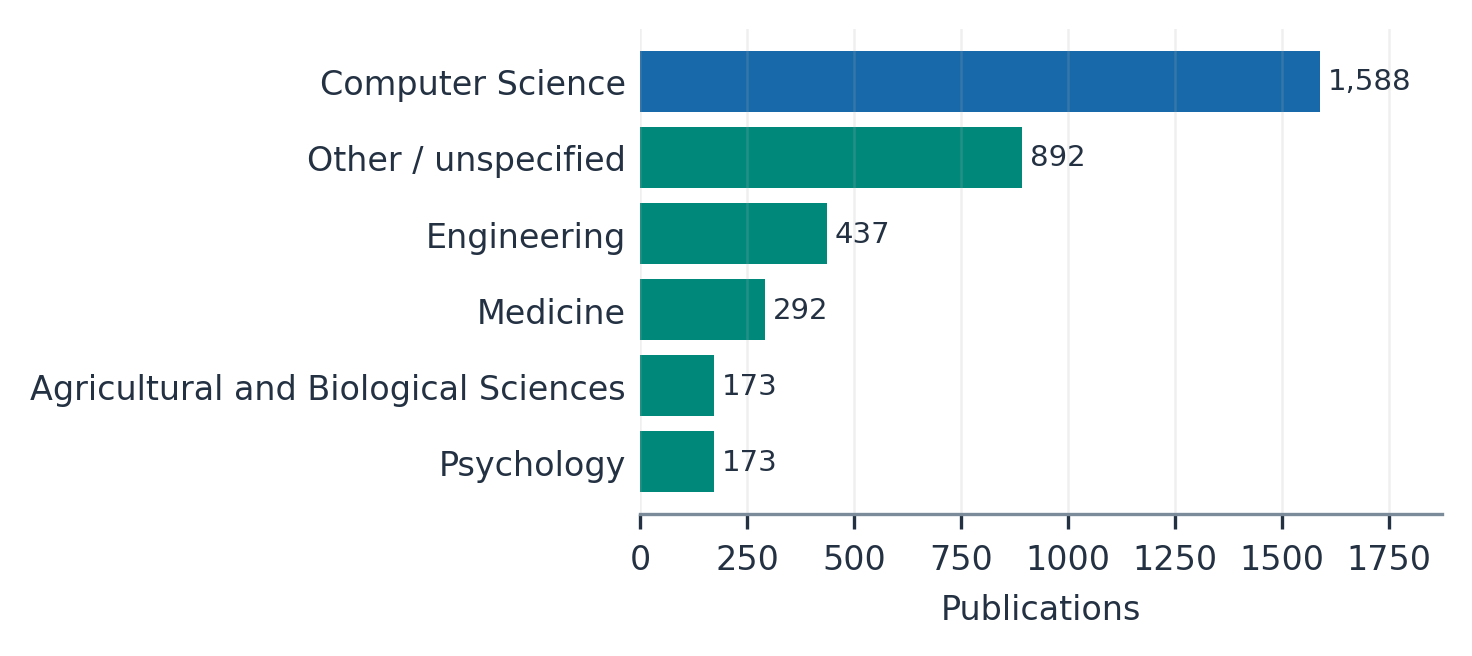
\includegraphics[width=\columnwidth]{figures/field_distribution.png}
  \caption{Primary-field distribution. ``Other / unspecified'' aggregates the remaining fields and 74 missing labels.}
  \label{fig:fields}
\end{figure}

Conference-oriented outputs dominate: proceedings articles constitute 1,459 records (41.0\%) and conference papers another 1,010 (28.4\%). Articles and journal articles together account for 802 (22.6\%), with preprints (105), book chapters (82), reviews (32), and smaller types forming the remainder. Open-access status is recorded as closed for 2,619 works; among the other 936, gold (286), diamond (268), green (219), hybrid (89), and bronze (74) are represented. These labels are inherited or normalized from source metadata and do not replace licence-level verification.

\subsection{Audit Effects}
The final audit materially changed the corpus. A previous 3,706-work release candidate lost 151 unique rows: 47 had only ambiguous-institution ownership support, 107 were alternate versions, and one was non-AI as well as unsupported; the categories overlap. Twenty-four supplied abstract or keyword corrections were then applied and search fields regenerated. Prior to that audit, a larger 4,058-row candidate export had been partitioned into 3,706 retained and 352 excluded non-AI records. Reporting both stages makes the difference between semantic screening and release-level entity/ownership validation explicit.

The quality validator passed 16 of 16 gates. Every row has title, publication date, source provenance, AI label, and a numeric confidence or documented human-review value. There are no unresolved secondary review decisions, unsupported ambiguous-institution inclusions, absolute workstation paths in model identifiers, or duplicate keys under the release checks.

\subsection{Analytics and User Workflows}
The curated data model supports several workflows beyond a static publication count. A policy analyst can filter the corpus by year, field, subfield, institution, publication type, or open-access status and export the resulting records. Institution views compare output while retaining publication-level links, which makes a surprising aggregate traceable to the works that produced it. Researcher views expose printed-name and co-authorship information, with verified profiles kept distinct from automatically parsed names. Topic pages provide a cross-disciplinary entry point, and the collaboration view projects shared publications into an exploratory network. The interface presents data-quality context alongside these views so that coverage and completeness are visible during interpretation.

The API mirrors these tasks through endpoints for publications, search, researchers, institutions, topics, analytics, collaboration, quality summaries, and exports. Keeping public access read-only is intentional: curation decisions pass through authenticated administrative workflows instead of being altered by a visualization client. User reports, author claims, and proposed corrections are staged for review. When approved, corrections are stored as overlays that survive a new source harvest. This division preserves a reproducible source-derived layer while still permitting the living system to repair errors.

Attribution-sensitive features apply stricter rules than general browsing. A person claiming a profile selects the exact printed author occurrences associated with their publications; a matching name alone does not transfer every homonym's output. Administrators can inspect ORCID, email-domain, affiliation, and competing-claim evidence. Approved authors may maintain biographical and affiliation-history information, while publication corrections and new works remain moderated. Institution counts continue to use the affiliation attached to the publication year rather than a researcher's current employer, avoiding retrospective transfer of older output when a person moves.

These interfaces are analytical affordances, not causal indicators. Raw counts do not control for institution size, field publication norms, database age, contribution position, or citation opportunity. Collaboration edges indicate co-publication, not funding flows or project leadership. Similarly, the open-access summary describes source-reported status at collection time. The platform therefore exposes records and denominators instead of producing a single institutional score. Responsible downstream studies should define their unit of analysis, freeze a dataset version, state filters, and report missingness before drawing comparative conclusions.

\section{Discussion}
\subsection{What the Workflow Adds}
The central design choice is separation of concerns. Discovery asks whether a source can supply a candidate; ownership asks whether evidence supports Sri Lankan participation; AI classification asks whether the intellectual content is relevant; deduplication asks what constitutes one countable work. Collapsing these questions into a single database query would make errors difficult to diagnose. Retaining separate evidence and decisions makes exclusion reasons auditable and allows each policy to evolve independently.

The uncertainty band also turns a model weakness into an operational queue. A binary classifier must force borderline records to one side; routing reserves automation for stronger predictions and directs the remainder to human judgement. The completed 214-case queue demonstrates closure of the process, though not benchmark accuracy. More broadly, the 60\% multi-source share supports the premise that national research infrastructure benefits from source complementarity.

\subsection{Observed Failure Modes and Design Lessons}
The audit exposed four recurring failure modes. First, institution aliases can be lexically plausible but refer to an unrelated organization or to an affiliation that is not attached to the publication. The 47 ownership exclusions show why institution normalization must retain evidence rather than only a standardized label. Second, versions frequently cross system boundaries: a repository item, preprint, conference record, and publisher version can carry different identifiers and slightly different titles. DOI-only deduplication would leave such groups unresolved, while aggressive fuzzy-title matching could merge distinct papers. Connected candidate groups plus canonical review provide a conservative middle ground.

Third, AI-looking language is not always evidence of AI research. ``Smart'' devices, rule-based automation, classical signal processing, and ordinary statistical forecasting account for many hard negatives in the development audit. Adding every available metadata field did not necessarily help because broad topic labels can reinforce these superficial cues. This motivated a compact textual feature contract and a review route rather than a fully automatic keyword taxonomy. Fourth, author names are inadequate ownership evidence. Initials collide, transliteration and ordering vary, and a printed author may change institution. The departmental roster validation therefore requires full-name or persistent-identifier support plus publication-time affiliation and holds initials-only cases.

These findings suggest a general lesson for small national observatories: conservative precision should be optimized at the public boundary, while recall gaps should remain visible and repairable. False inclusion changes institutional statistics and public profiles; a documented omission can be added during the next incremental cycle. This asymmetry justifies the use of review queues, explicit retirement, and user feedback rather than one irreversible extraction run.

\subsection{Threats to Validity}
First, the corpus is not a census. Repository outages, incomplete affiliations, missing abstracts, source lag, and unindexed local venues can reduce recall. The departmental validation found conservative attributions but also exposed missing upstream coverage. A national recall study would require authoritative staff and publication lists across institutions.

Second, affiliation-based ownership is a policy construct. It may omit diaspora work without qualifying publication-time Sri Lankan evidence and can include internationally conducted work when the documented project ownership rule passes. The policy is reproducible but should not be read as nationality or residency.

Third, source-provided topic, field, language, open-access, and document-type labels inherit upstream errors. The 11,585 author strings are not 11,585 verified people. ORCID coverage is incomplete, and name disambiguation remains an active problem. Fourth, the rapid annual increase mixes real growth with changing coverage; 2026 is incomplete. Finally, operational labels were created during system development and curation. Without independently blinded annotation, overlap, inter-annotator agreement, and a frozen test protocol, classifier metrics would overstate the evidence.

\subsection{Responsible Release}
The canonical package retains abstracts for 2,896 records. Although most bibliographic metadata can be broadly reused, source-level rights for every retained abstract are not consistently encoded. Consequently, the dataset is technically finalized but not yet cleared for unrestricted public deposition. Before release, the project must finish field-level rights review, select a dataset licence, and replace the pending licence marker. This restriction does not prevent peer review of the method, aggregate results, source code, schemas, and audit procedure, but reviewers should request controlled access if row-level inspection is required.

\balance
\section{Conclusion and Future Work}
ResearchLanka AI demonstrates that a useful national AI research map requires more than keyword search. By combining multi-source harvesting, common-schema transformation, conservative ownership evidence, version-aware deduplication, uncertainty-aware AI triage, and explicit human adjudication, the pipeline produces a 3,555-work corpus with measurable completeness and no residual duplicates under its release checks. The same data layer supports a reproducible package, API, and interactive analytics interface.

Future work should prioritize an independently blinded benchmark with multiple annotators and agreement reporting; institution-by-institution recall studies against official publication lists; persistent person and organization identifiers; temporal version graphs rather than canonical-only works; and source-field licence automation. After rights clearance, the versioned corpus and model artifact can be deposited with a permanent identifier. The architecture is deliberately configurable so that the evidence policies and adapters can be reused for other national or thematic research observatories.

\section*{Acknowledgment}
The author thanks the maintainers of OpenAlex, Crossref, SLJOL, and participating institutional repositories. Any source attribution or classification errors remaining in the release are the responsibility of the ResearchLanka AI project.

\bibliographystyle{ieeetr}
\bibliography{references}

\end{document}
